%	!Mode::"UTF-8"
%	本模板设置改自北京大学交叉学院 王宇哲学长和北京大学化学与分子工程学院 王应泽同学的分享,特此感谢!
%	模板制作:北京大学化学与分子工程学院 王梓涵
%	Email:2100011837@stu.pku.edu.cn
%	本模板仅适用于北京大学物理化学实验报告,其他学校请自行修改
%	吐槽:Latex用于写物化实验报告还是过于繁琐了,不过还是比Word好用多了(๑•̀ㅂ•́)و✧ (此吐槽由copilot自动生成,模板作者认为word更好用)
%	本模板仅供交流学习使用,不可用作商业用途。

\documentclass[12pt]{article}

%	页面设置
\usepackage{geometry}
\geometry{left=2.5cm, right=2.5cm, top=2.5cm, bottom=2.5cm}
\usepackage{graphicx}
\usepackage{ctex}
\usepackage{fontspec}
\usepackage{setspace}
\usepackage[usenames,dvipsnames]{xcolor}
\usepackage{titlesec}

%	字体设置
\setmainfont{Times New Roman}
\setCJKmainfont{SimSun}
\setCJKsansfont{SimHei}
\setCJKmainfont[AutoFakeBold=true]{SimSun}

%	表格设置\
\usepackage{array,colortbl}
\usepackage{makecell}
\newcommand{\addcell}[2][4]{\makecell{\zihao{#1}\textsf{#2}}}
\usepackage{titlesec}
\usepackage{booktabs}
\usepackage{ragged2e} 
\usepackage{multirow}
\usepackage{tabularx}

%	设置图注、表注
\usepackage{caption}
\usepackage{bicaption}
\captionsetup{labelsep=quad, font={small, bf}, skip=2pt}
\DeclareCaptionOption{english}[]{
    \renewcommand\figurename{Fig.}
    \renewcommand\tablename{Table}
}
\captionsetup[bi-second]{english}

%	设置页眉
\usepackage{fancyhdr}
\usepackage{xpatch}
\pagestyle{fancy}
\fancypagestyle{preContent}{
    	\fancyhead[L]{\zihao{-5} 物理化学实验}
    	\fancyhead[C]{\zihao{-5} 实验七\ \ 氢氧化铁溶胶的制备及其性质的研究}
    	\fancyhead[R]{\zihao{-5} 2100011837\ 王梓涵}
		\renewcommand{\headrulewidth}{2pt}
		\renewcommand{\footrulewidth}{1pt}
		\xpretocmd\headrule{\color{BrickRed}}{}{\PatchFailed} % 设置页眉分割线颜色
		\xpretocmd\footrule{\color{BrickRed}}{}{\PatchFailed} % 设置页脚分割线颜色
}
\pagestyle{preContent}



%	设置首页页眉及取消首页页脚 若不需要首页页眉 请注释掉下列内容
\fancypagestyle{plain}{
	\fancyhead[L]{\zihao{-5} 物理化学实验}
    \fancyhead[C]{\zihao{-5} 实验七\ \ 氢氧化铁溶胶的制备及其性质的研究}
	\fancyhead[R]{\zihao{-5} 2100011837\ 王梓涵}
	\cfoot{}
}

%	设置标题格式
\titleformat*{\section}{\color{Mahogany}\zihao{4}\sffamily}
\titleformat*{\subsection}{\zihao{-4}\sffamily}
\titleformat*{\subsubsection}{\zihao{-4}\sffamily}
\titlespacing*{\section}{0pt}{10pt}{10pt}
\titlespacing*{\subsection}{0pt}{10pt}{5pt}
\titlespacing*{\subsubsection}{0pt}{10pt}{5pt}


%	设置引用格式(ACS格式规范)
%	注意:请安装JabRef
%	JabRef使用参考:https://blog.csdn.net/weixin_44191286/article/details/85698921
\usepackage[super,round,comma,compress]{natbib}

%	数学公式增强
\usepackage{amsmath}
\usepackage{amssymb}

%	单位与数学式
\usepackage{siunitx}

%	设置封面
\begin{document}
    % 标题页
    \begin{titlepage}
    	% 页眉
    	\thispagestyle{plain}
        % 校徽图片
        \begin{figure}[h]
            \centering
            \includegraphics{pku.png}
        \end{figure}
        \vspace{24pt}
        % 标题
        \centerline{\zihao{-0} \textsf{\textcolor{Mahogany}{物理化学实验报告}}}
        \vspace{40pt} % 空行
        \begin{center}
            \begin{tabular}{cp{14.1cm}}
                % 题目
                \addcell[2]{题目:} & \addcell[2]{氢氧化铁溶胶的制备及其性质的研究} \\
                \cline{2-2}
            \end{tabular}
        \end{center}
        \vspace{20pt} % 空行
        \begin{center}
            \doublespacing
            \begin{tabular}{cp{5cm}}
                % 姓名
                \addcell{姓\phantom{空格}名:\ } & \addcell{王梓涵} \\
                \cline{2-2}
                % 学号
                \addcell{学\phantom{空格}号:\ } & \addcell{2100011837}\\
                \cline{2-2}
                % 组别
                \addcell{组\phantom{空格}别:\ } & \addcell{22组} \\
                \cline{2-2}
                % 实验日期
                \addcell{实验日期:\ } & \addcell{2023.11.9}\\
                \cline{2-2}
                % 室温
                \addcell{室\phantom{空格}温:\ } & \addcell{294.00\ K}\\
                \cline{2-2}
                % 大气压强
                \addcell{大气压强:\ } & \addcell{102.34\ kPa}\\
                \cline{2-2}
            \end{tabular}
            \begin{tabular*}{\textwidth}{c}
                \\ % 这是空行
                \\ % 这是空行
                \\ % 这是空行
                \hline % 分割线
            \end{tabular*}
        \end{center}
        % 摘要
        \textsf{\textcolor{BrickRed}{摘\ \ 要}}\ \ 本实验使用凝结法制备了$\rm Fe(OH)_{3}$溶胶,并利用热渗析法对其进行了初步纯化,使$\rm Fe(OH)_{3}$溶胶电导降为$128\  {\rm \mu S\cdot cm^{-1}}$。本实验还利用上一组同学制备的电导为$17.7\ \ {\rm \mu S\cdot cm^{-1}}$的$\rm Fe(OH)_{3}$溶胶进行电泳实验,通过溶胶电泳实验,计算得溶胶电动电势$\zeta=(0.0525\pm 0.0003)\ \ {\rm V}$,最后分析了实验不完全成功的原因,提出了实验的改进方案。
        \\
        \\
        % 关键字
        \textsf{\textcolor{BrickRed}{关键词}}\ \ 氢氧化铁;溶胶制备;溶胶电泳;Zeta电势
    \end{titlepage}

    \section{引言}
		\subsection{实验目的}
			本实验的实验目的主要有以下几点\cite{physchemlab}:\par
			\ \ \ \ \ \ \ \ 1. 了解溶胶的性质、特点、制备方法及原理。\par
			\ \ \ \ \ \ \ \	2. 用凝结法制备胶体并用热渗透进行分离纯化。\par
			\ \ \ \ \ \ \ \	3. 掌握界面移动电泳及其原理。\par
		\subsection{实验原理和实验方法}
		本实验使用凝结法制备氢氧化铁胶体,具体的胶体性质、实验原理和实验方法在实验预习报告中如\textbf{图1}所示: \par
		\begin{figure}[h]
			\centering
			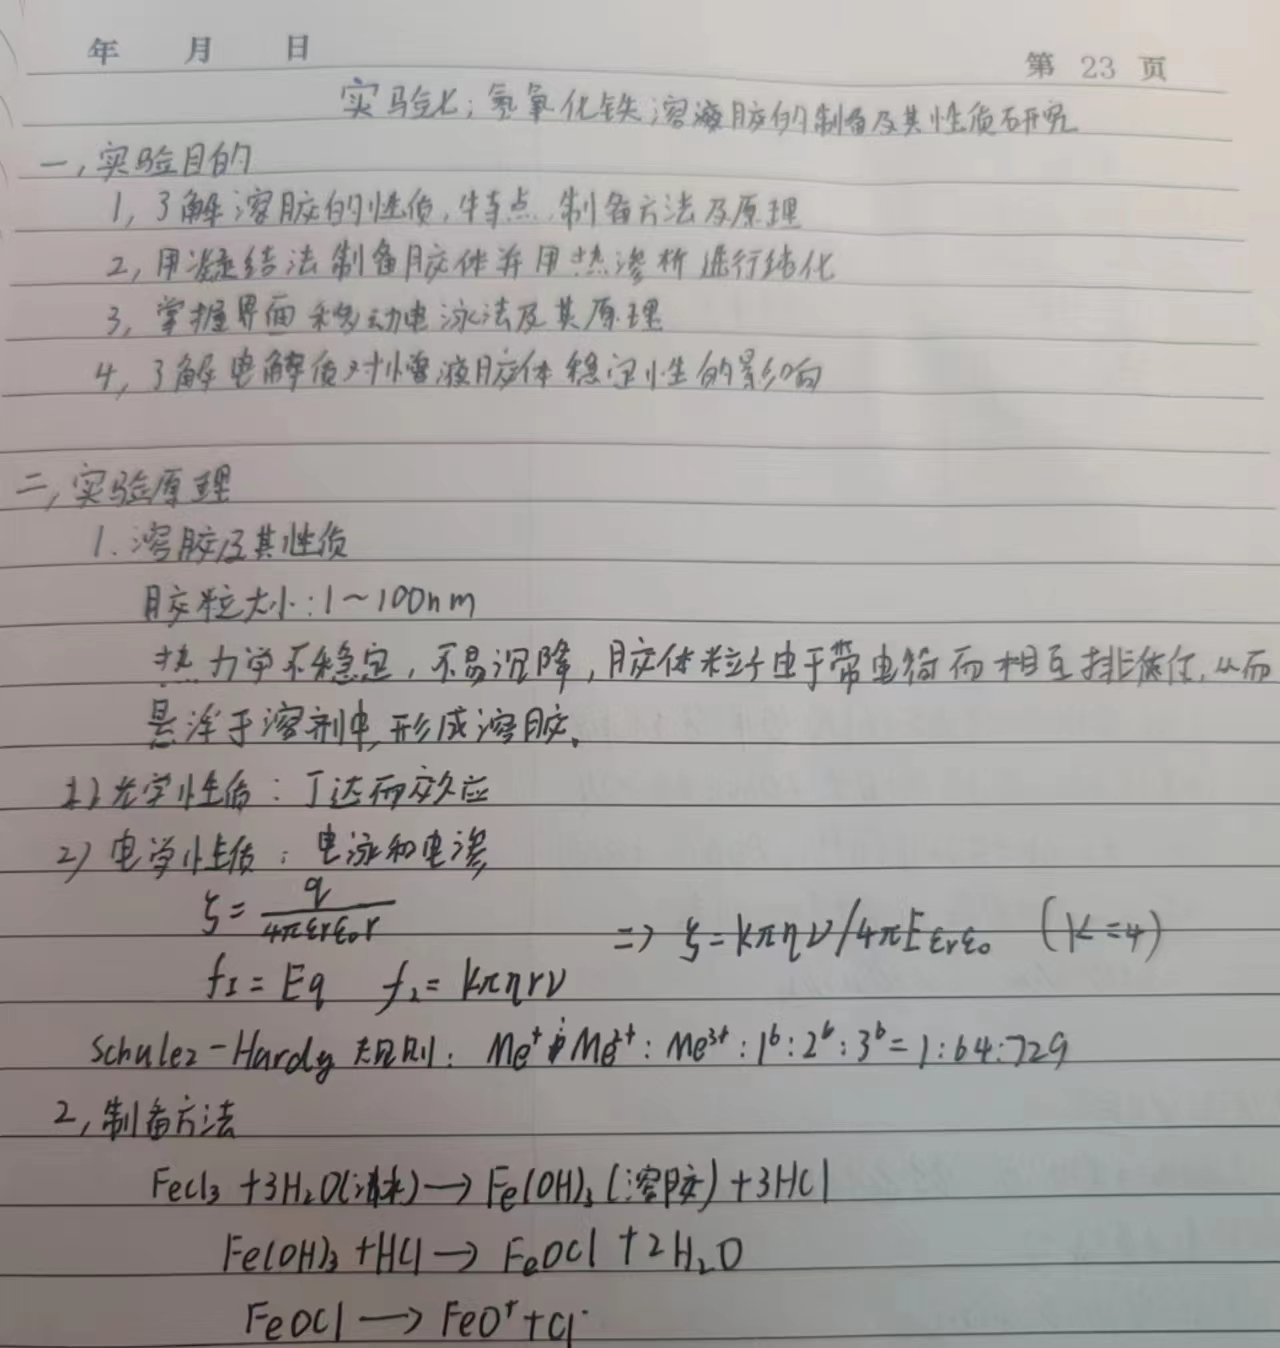
\includegraphics[width=0.8\textwidth]{1.png}
			\bicaption{实验预习报告的实验原理部分}{The principle part of the experiment in the experiment preview report}
		\end{figure}
			
	     
    \section{实验部分}
    	\subsection{仪器和试剂}
    		仪器:滴管,单口烧瓶,烧杯,试管,$\rm 5 mL$量筒,透析袋夹子,U型电泳管,稳压电泳仪,铂电极,秒表,透析袋。\par
			试剂:\ \  $\rm FeCl_{3}$溶液$(10\%)$,$\rm AgNO_{3}$溶液$0.01\ \ {\rm mol\cdot dm^{-3}}$,$\rm KSCN$溶液$0.1\ \ {\rm mol\cdot dm^{-3}}$,$\rm KCl$溶液$0.08\ \ {\rm mol\cdot dm^{-3}}$。\par 
    			
    	 \subsection{实验内容}
		 本实验的实验操作如下所示,其中笔者的思考和具体实验中的不同操作会在括号中写出。\par
		 \subsubsection{$\rm Fe(OH)_{3}$溶胶的制备}
		 	在洁净的$\rm 250 \ \ mL$单口烧瓶中加入$\rm 100 \ \ mL$去离子水与搅拌磁子,加热至沸。一边搅拌一边缓慢滴加$\rm 5.0\ \ mL \ \ 10\% \ \ FeCl_{3}$溶液,加完后保持微沸状态继续搅拌加热$\rm 10\ \ min$,得到红棕色的氢氧化铁溶液。过程中不可补加水。(具体实验装置如\textbf{图2}所示)
			 \begin{figure}[h]
				\centering
				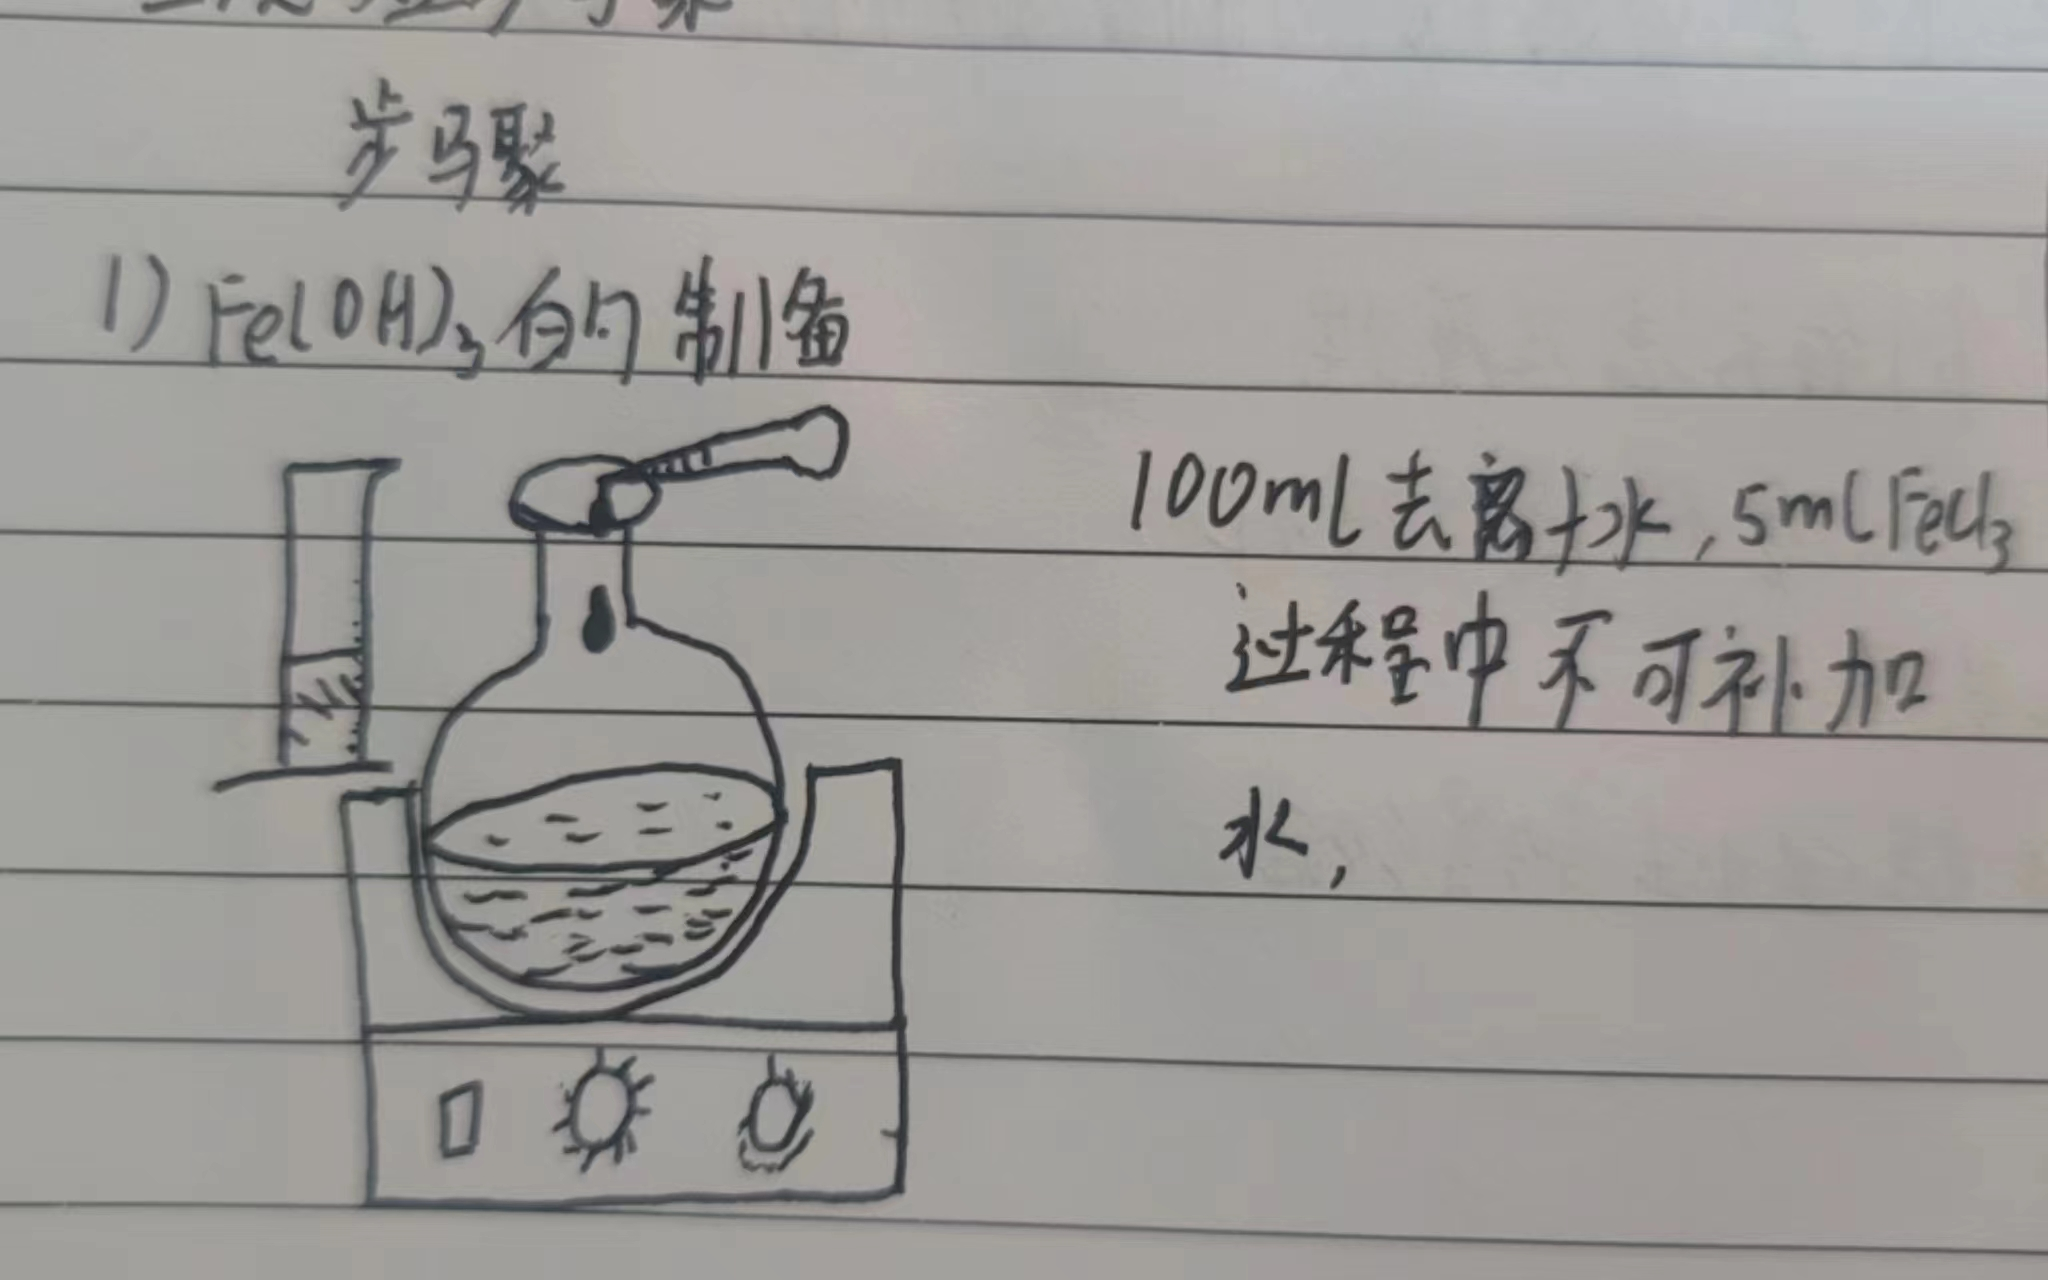
\includegraphics[width=0.6\textwidth]{2.png}
				\bicaption{溶胶制备装置}{Sol preparation device}
			\end{figure}
		 \subsubsection{$\rm Fe(OH)_{3}$溶胶的纯化}
			1. 将剪好的透析袋在去离子水中浸泡至变柔软,将透析袋一端用夹子夹好,装入去离子水试漏,浸泡在去离子水中备用。\par 
			2. 将制得的氢氧化铁溶胶倒入透析袋中,并将透析袋另一端用夹子夹好并测试是否有漏液。将密封好的透析袋置于装有已预热去离子水$\rm (60\sim 80\ \ ^{\circ }C)$的$\rm 1000\ \ mL$烧杯中,在电磁搅拌下进行透析。尽可能使透析袋转动起来以提高透析效率。\par 
			3. 在透析的前一个小时中,每隔$\rm 30\ \ min$更换一次水(水事先在水浴锅中预热备用)。第二次换水用$\rm KSCN$溶液检测透析液中的$\rm Fe^{3+}$离子,用$\rm AgNO_{3}$溶液检测$\rm Cl^{-}$离子,直至透析液中的$\rm Cl^{-}$离子浓度基本检测不出来为止,改为使用电导率仪测量透析液的电导率变化来监测透析速度,当电导率变化缓慢时可更换新的去离子水(\textbf{因为烧杯中的透析液在高速旋转,因此直接即将电导仪插入正在透析的体系会使得仪器示数剧烈波动,因此用电导率仪测量透析液电导率和用$\rm AgNO_{3}$溶液检测$\rm Cl^{-}$离子一样是在换水间隙完成的})。直至透析液电导$<\rm 30 \ \ μS/cm$,再用
			电导率仪测量溶胶的电导率。\par
			4. 将装有溶胶的透析袋置于盛有新换去离子水的烧杯中,并将写好溶胶电导值、姓名、学号信息的标签纸贴于该烧杯内壁。烧杯杯口用保鲜膜密封。放在指定位置储存,供下周实验的同学使用(\textbf{感觉在标签上记录溶胶电导值是没有意义的,因为在我们离开后透析纯化也依然在进行,在进行溶胶电泳实验中上一组同学记录的数据和我们试剂测量的数据就有较大不同})。
			\vbox{\ \ }
			\vbox{\ \ }
			\subsubsection{溶胶电泳实验}
				1. 配制电导值与溶胶电导值相同的$\rm KCl$溶液作为辅助液,用电导率仪测量辅助液电导率值为$17.8\ \ {\rm \mu S/cm}$。\par 
				2. 彻底清洗电泳管至内壁不挂水珠,用去离子水洗3次,再用少量溶胶润洗2次(\textbf{在实际操作过程中并没有使用溶胶润洗,这有两方面考量,一方面我们的溶胶量不太够,另一方面溶胶润洗会有较严重的挂壁并模糊刻度,为后续的电泳读数造成较大的困难。因此在此处我们是采用辅助液进行润洗});将电泳管固定在支架上,从中间管加溶胶至刻度$\rm 4\ \ cm$附近(\textbf{我们的溶胶无法支持滴加至4cm刻度,其本身影响不大,但这确实是导致最后溶胶电泳实验不完全成功的原因之一});用滴管交替向左右两管沿管壁小心滴加辅助液,直至液面达刻度$\rm 8\sim 9\ \ cm$。开始加辅助液时较慢,使液滴沿管壁流下,防止液面振荡。当发生液面振荡界面模糊,应立即停下来,等稳定后再加。当液面高度离界面较高时,可适当加快滴加速度。\par 
				3. 将电极插入电泳仪的“+”、“-”插孔中,打开电泳仪预热。将两电极插入装有辅助液的烧杯中,调节两极间电压稳定在$\rm 100\pm 5\ \ V$。断开回路,小心地将电极插入电泳管中大约液面下$1\ \ \rm cm$,正极插入左管,负极插入右管,记录电极位置和界面位置。连通电路开始电泳实验并计时。观察溶胶与辅助液的界面位置,每隔$\rm 1\ \ min$记录正极和负极的界面位置,测6组以上数据,同时观察并记录界面状态以及电极表面的变化。\par 
				4. 测完后关闭电源,用软尺沿电泳管的中心线测量两电极间距离,测量三次取平均值,计算电动电势。
	
	 \section{数据与结果}
 		\subsection{实验数据记录及处理}
 			\subsubsection{$\rm Fe(OH)_{3}$溶胶的纯化}
			 记录$\rm Fe(OH)_{3}$溶胶纯化过程中更换水的次数、时间间隔及离子检测结果,检测不出$\rm Cl^{-}$后用电导率仪测量并记录每次换水时透析液及最后溶胶的电导率,结果如\textbf{表1}所示,其中“$+$”表示离子检出,“$-$”表示粒子未检出。
		 		
			 \begin{table}[h]
				\centering
				\zihao{5}
				\bicaption{$\rm Fe(OH)_{3}$溶胶的纯化过程}{Purification process of $\rm Fe(OH)_{3}$ sol}
				\begin{tabular}{cccccc}
					\toprule
					编号 & 透析时长$t/{\rm min}$ & ${\rm Cl^{-}}$检测 & ${\rm Fe^{3+}}$检测 & 透析液电导/${\rm \mu S\cdot cm^{-1}}$ & 胶体电导/${\rm \mu S\cdot cm^{-1}}$  \\
					\midrule
					1 & 20.0 & $+$ & $-$ &  & \\
					2 & 20.0 & $+$ & $-$ &  &\\
					3 & 20.0 & $+$ & $-$ &  &\\
					4 & 30.0 & $+$ & $-$ &  &\\
					5 & 30.0 &$-$ & $-$& 43.2 &\\
					6 & 30.0 &$-$ & $-$& 10.4 & 162\\
					7 & 30.0 &$-$ & $-$& & 128\\
					\bottomrule
				\end{tabular}
			\end{table}
			\par
			\subsubsection{溶胶电泳实验与两电极间距离的测量}
			在$\rm Fe(OH)_{3}$溶胶电泳实验过程中,记录正负两极的界面位置随时间的变化,结果如\textbf{表2}所示,但因实验操作的原因,我们只得到了右侧界面的数据,具体导致这的原因将在实验误差中详细分析。
			\begin{table}[h]
				\centering
				\zihao{5}
				\bicaption{$\rm Fe(OH)_{3}$溶胶电泳实验数据}{$\rm Fe(OH)_{3}$ sol electrophoresis experimental data}
				\begin{tabular}{cccc}
					\toprule
					编号 & $t/{\rm s}$ & $h_{L}/{\rm cm}$ & $h_{R}/{\rm cm}$  \\
					\midrule
					1 & $0$ & $2.10$ & $2.15$  \\
					2 & $60$ & $-$ & $2.85$  \\
					3 & $151$ & $-$ & $3.15$  \\
					4 & $184$ & $-$ & $3.23$  \\
					5 & $248$ & $-$ & $3.30$  \\
					6 & $301$ & $-$ & $3.38$  \\
					7 & $362$ & $-$ & $3.49$  \\
					8 & $424$ & $-$ & $3.60$  \\
					9 & $484$ & $-$ & $3.71$  \\
					10 &$545$ & $-$ & $3.83$  \\
					11 &$601$ & $-$ & $3.99$  \\
					12 &$659$ & $-$ & $4.09$  \\
					\bottomrule
				\end{tabular}
			\end{table}
			\par
		在$\rm Fe(OH)_{3}$溶胶电泳实验进行过程中,观察界面状态以及电极表面的变化。随着电泳实验的进行,右侧界面明显变得更加清晰;两侧电极表面有少量气泡产生,右侧比左侧产生的气泡更多。\par 
		测量完成后关闭电源,用软尺沿电泳管的中心线测量两电极间的距离$l$,测量分为三部分,分别为左侧电极距离刻度底端的长度$l_{L}$、右侧电极距离刻度底端的长度$l_{R}$以及底部U形区域的长度$l_{M}$,三者加和即可得到$l$,重复测量三次,结果如\textbf{表3}所示。
		\begin{table}[h]
			\centering
			\zihao{5}
			\bicaption{两电极间距离测量数据}{Measurement data of distance between two electrodes}
			\begin{tabular}{ccccc}
				\toprule
				编号 & $l_{L}$ & $l_{R}$ & $l_{M}$&$l_{all}$  \\
				\midrule
				 1&4.95&4.65&7.20&16.80  \\
				 2&4.95&4.65&7.40&17.00  \\
				 3&5.00&4.60&7.55&17.15  \\
				\bottomrule
			\end{tabular}
		\end{table}
		\par
		计算两电极间距离$l$的平均值为:
		$$
		l = \frac{l_{all,1}+l_{all,2}+l_{all,3}}{3} = \frac{16.80+17.00+17.15}{3} = 16.98 
		$$
		两电极间距离$l$的不确定度为:
		$$
		\sigma_{l} = \sqrt{\frac{\sum_{i=1}^{3}(l_{all,i}-l)^{2}}{3(3-1)}} = \sqrt{\frac{(16.80-16.98)^{2}+(17.00-16.98)^{2}+(17.15-16.98)^{2}}{3(3-1)}} = 0.11
		$$
		因此
		$$
		l = (16.98\pm0.11)\ \ \rm cm
		$$
		\subsubsection{胶体界面时间-迁移距离关系图与平均泳动速度计算}
		$\rm Fe(OH)_{3}$胶体右侧界面迁移距离为:
		$$
		s_{R}=h_{R}-h_{R_{0}}
		$$
		其中$h_{R_{0}}$为右侧界面初始位置,为$2.15\ \ \rm cm$。\par
		根据以上公式及\textbf{表2}数据,计算左右两侧胶体界面的迁移距离随时间$t$的变化,结果如\textbf{表4}所示。
		\begin{table}[h]
			\centering
			\zihao{5}
			\bicaption{胶体界面迁移距离随时间的变化}{The change of colloidal interface migration distance with time}
			\begin{tabular}{cccc}
				\toprule
				编号 & $t/{\rm s}$ & $s_{L}/{\rm cm}$ & $s_{R}/{\rm cm}$  \\
				\midrule
				1 & $0$ & $-$ & $0.00$  \\
				2 & $60$ & $-$ & $0.70$  \\
				3 & $151$ & $-$ & $1.00$  \\
				4 & $184$ & $-$ & $1.08$  \\
				5 & $248$ & $-$ & $1.15$  \\
				6 & $301$ & $-$ & $1.23$  \\
				7 & $362$ & $-$ & $1.34$  \\
				8 & $424$ & $-$ & $1.45$  \\
				9 & $484$ & $-$ & $1.56$  \\
				10 &$545$ & $-$ & $1.68$  \\
				11 &$601$ & $-$ & $1.84$  \\
				12 &$659$ & $-$ & $1.94$  \\
				\bottomrule
			\end{tabular}
		\end{table}
		\par
		根据\textbf{表4}数据作出$s_{R}-t$关系的散点图,并用origen对其进行线性拟合,作出拟合直线,如\textbf{图3}所示。
		\begin{figure}[!h]
			\centering
			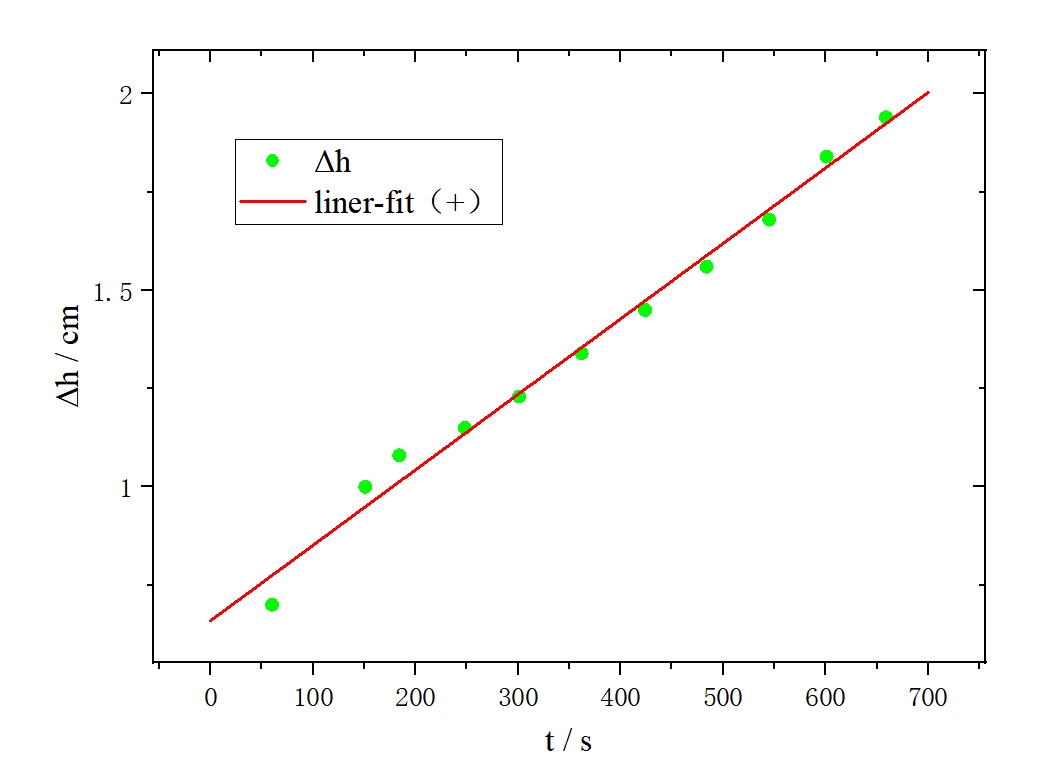
\includegraphics[width=0.80\textwidth]{3.png}
			\bicaption{$\rm Fe(OH)_{3}$溶胶电泳时间$t$-界面迁移距离$s$关系图}{$s-t$ Diagram of $\rm Fe(OH)_{3}$ sol electrophoresis interface}
		\end{figure}
		\par
		拟合直线的方程为:
		$$
		s_{R}/{\rm cm}=(0.00192\pm 0.000007)t/{\rm s}+(0.6595\pm 0.021),\   \  R=0.9874
		$$
		\par
		可以注意到直线的截距并不为零,这是因为,我们在打开电泳仪电源后,\textbf{并未及时开始计时,因而凝胶存在一个初始的位移},因此我们在拟合直线时,第一个数据点以前的数据舍去,以确保数据的准确。\par
		拟合直线的斜率即为界面迁移的平均速度,即:
		$$
		v_{R} = (0.00192\pm 0.000007)\ \ \rm cm/s
		$$
		\subsubsection{电动电势的计算}
		利用公式:
		$$
		\zeta=\frac{\eta s l}{\varphi t \varepsilon_{r} \varepsilon_{0}}=\frac{\eta v l}{\varphi  \varepsilon_{r} \varepsilon_{0}}
		$$
		\par
		计算$\rm Fe(OH)_{3}$胶体的电动电势,其中两电极间距离$l=(16.98\pm 0.11){\rm cm}$,平均泳动速度(界面迁移平均速度)$v=(0.00192\pm 0.00007)\ \ {\rm cm\cdot s^{-1}}$,两电极间电势差$\varphi=100\ \ {\rm V}$。\par
		查阅\textit{CRC Handbook of Chemistry and Physics}\citealp{crc},得到真空介电常数$\varepsilon_{0}=8.8542\times 10^{-12}\ \ {\rm F\cdot m^{-1}}$,$20\ \ {\rm ^{\circ}C}$时水的相对介电常数$\varepsilon_{r}=80.10$;\par
		查阅《物理化学实验(第四版)》书后附录表D.4-15\citealp{textbook},知$t=20.2\ \ {\rm ^{\circ}C}$时,水的黏度$\eta=1.000\ \ {\rm mPa\cdot s}$,$t=21\ \ {\rm ^{\circ}C}$时,水的黏度$\eta=0.981\ \ {\rm mPa\cdot s}$,实验室实际温度$t=20.85\ \ {\rm ^{\circ}C}$,近似认为$20.2\ \ {\rm ^{\circ}C\sim 21\ \ ^{\circ}C}$范围内水的黏度与温度呈线性关系,计算$t=17.6\ \ {\rm ^ {\circ}C}$时水的黏度为:
		$$
		\eta=0.981+\frac{1.000-0.981}{21-20.2}\times (20.85-20.2)\ \ {\rm mPa\cdot s}=0.9964\ \ {\rm mPa\cdot s}
		$$
		代入各项数据,得:
		$$
		\zeta=\frac{\eta v l}{\varphi  \varepsilon_{r} \varepsilon_{0}}=\frac{0.9964\ \ {\rm mPa\cdot s} \times 1.92\times 10^{-3}\ \ {\rm cm\cdot s} \times 16.98\ \ {\rm cm}}{100\ \ {\rm V}  \times 80.10 \times 8.8542\times 10^{-12}\ \ {\rm F\cdot m^{-1}}}=0.0525\ \ {\rm V}
		$$
		不确定度$\sigma_{\zeta}$为:
		$$
		\sigma_{\zeta}=\zeta\sqrt{\frac{\sigma_{l}^{2}}{l^{2}}+\frac{\sigma_{v}^{2}}{v^{2}}}=0.0525 {\rm V}\times\sqrt{\frac{(0.11\ \ {\rm cm})^{2}}{(16.98\ \ {\rm cm})^{2}}+\frac{(0.00007\ \ {\rm cm\cdot s^{-1}})^{2}}{(0.00192\ \ {\rm cm\cdot s^{-1}})^{2}}}=0.00194\ \ {\rm V}
		$$
		因此
		$$
		\zeta=(0.0525\pm 0.00194)\ \ {\rm V}
		$$
 	\section{讨论与结论}
	 \subsection{误差与误差分析}
		\subsubsection{实验误差}
		在计算电动电势的过程中,$\sigma_{l}$和$\sigma_{v}$都对电动电势的不确定度$\sigma_{\zeta}$造成了贡献。其中电极间距$l$的贡献为:
		$$
		\frac{\sigma_{l}^{2}}{l^{2}} / \frac{\sigma_{\zeta}^{2}}{\zeta^{2}} = \frac{(0.11\ \ {\rm cm})^{2}}{(16.98\ \ {\rm cm})^{2}} / \frac{(0.00194\ \ {\rm V})^{2}}{(0.0525\ \ {\rm V})^{2}} = 3.07\%
		$$
		平均泳动速度$v$的贡献为:
		$$
		\frac{\sigma_{v}^{2}}{v^{2}} / \frac{\sigma_{\zeta}^{2}}{\zeta^{2}} = \frac{(0.00007\ \ {\rm cm\cdot s^{-1}})^{2}}{(0.00192\ \ {\rm cm\cdot s^{-1}})^{2}} / \frac{(0.00194\ \ {\rm V})^{2}}{(0.0525\ \ {\rm V})^{2}} = 97.34\%
		$$
		\subsubsection{电泳实验不完全成功的原因以及误差来源}
		由误分析可见电动电势的不确定度主要是由电泳速度$v$的不确定度造成的。而本次实验我们在电泳的操作上确实存在较多问题,导致电泳速度的不确定度较大,这里集中进行讨论。\par
		实验不完全成功的原因:\par
		\begin{enumerate}
			\item \textbf{溶胶量不足}:因为一些原因我们获得的溶胶量不足,同时也因为我们自己的失误浪费了一定量的溶胶,这导致我们在将溶胶装入U形管中时,溶胶的高度只有$2.5\ \ \rm cm$,而实验要求的高度为$4\ \ \rm cm$,这一来增大了我们需要滴加的辅助液的量,同时也减小了我们两电极的距离,使得可能存在一定的误差。同时较少的溶胶量也减少了实验的容错率,当我们在左侧管滴加辅助液以获得清晰界面的尝试失败后,我们很难进行有效的补救措施,如吸走一部分溶胶。\par
			\item \textbf{滴定液面失败}:导致我们失去左侧数据的元凶就是我们在试图缓慢滴加缓冲液时,并未形成清晰的界面,这导致左侧的度数变得极其困难,因而无法获得左侧数据。
		\end{enumerate}
		实验的误差来源:\par
		\begin{enumerate}
			\item \textbf{移动速度并非匀速}:在计算时,我们假设溶胶界面的上升时速度是匀速的,但实际上电泳过程中界面迁移并非匀速,而是由静止状态逐渐开始迁移的,因此我们拟合得到的界面迁移速度与稳恒状态时的界面迁移速度有所不同。\par
			\item \textbf{界面读数困难}:在电泳过程中,胶体与辅助液的分界面不够清晰,溶胶界面在上升时并非保持一个平稳的状态,其会有不小幅度的波动,因此再读数时可能会引入不小的误差\par
			\item \textbf{时间不准确}:实验过程中读取界面迁移距离$s$和从计时器读取时间$t$不完全同步,两者有时间上的先后,且每次测量时情况不同,导致$s-t$图直线的位置发生偏移,误差变大。\par
		\end{enumerate}
		\subsection{实验现象}
		\subsubsection{溶胶纯化实验现象}
		我们注意到,在透析纯化的过程中铁离子几乎不会进入透析液中,因此在透析过程中,透析液应当为几乎澄清的状态,若出现较大的染色,则说明透析袋可能存在密封问题。\par
		\subsubsection{电泳实验现象}
		在电泳实验过程中,我们观察到了以下现象:\par
		\begin{enumerate}
			\item \textbf{界面变化}:在进行凝胶电泳的过程中我们发现,随着电泳的进行,胶体与辅助液的分界面逐渐变得清晰,我们推测这是因为在电场的作用下,胶体中的粒子会向着电极移动,而胶体中的粒子在移动时会与溶液中的水分子发生碰撞,这些碰撞会使得溶胶分子被压紧形成更加清晰的液面。左侧液面变清晰的原因也有可能是在电泳过程中凝胶在电场的作用下自动产生了聚集。\par
			\item \textbf{电极反应}:随着电泳进行,正负极铂电极上均出现气泡,且负极上气泡更多。这非常好理解,因为在电解水的过程中,正极上会产生氧气,负极上会产生氢气,因此在电泳过程中,电极上会产生气泡。\par
		\end{enumerate}	
 		\subsection{实验结论}
		 本实验使用凝结法制备了$\rm Fe(OH)_{3}$溶胶,利用热渗析法对其进行了初步纯化,使$\rm Fe(OH)_{3}$溶胶电导降为$128\  {\rm \mu S\cdot cm^{-1}}$。利用上一组同学制备的电导为$17.7\ \ {\rm \mu S\cdot cm^{-1}}$的$\rm Fe(OH)_{3}$溶胶进行电泳实验,通过溶胶电泳实验,计算得溶胶电动电势$\zeta=(0.0525\pm 0.0003)\ \ {\rm V}$,分析了实验不完全成功的原因,提出了实验的改进方案。

\vbox{}  
%参考文献
\bibliographystyle{unsrt}
\bibliography{cite}
\end{document}